\documentclass[12pt,a4paper]{article}
% XeLaTeX + ShareLaTeX 环境设置
\usepackage[UTF8,scheme=plain]{ctex}
\usepackage{geometry}
\geometry{a4paper,left=2.5cm,right=2.5cm,top=2.5cm,bottom=2.5cm}

% 基础宏包
\usepackage{amsmath}           % 数学公式
\usepackage{amssymb}          % 数学符号
\usepackage{graphicx}          % 图片支持
\usepackage{float}             % 浮动体设置
\usepackage{booktabs}          % 用于美观的表格边框
\usepackage{fancyhdr}          % 页眉页脚
\usepackage{lastpage}          % 获取总页数
\usepackage{zhnumber}          % 中文数字
\usepackage{subcaption}        % 支持子图
\usepackage{placeins}          % 用于\FloatBarrier命令
\usepackage{indentfirst}       % 确保章节后第一段也缩进

% 参考文献设置 - 适用于ShareLaTeX + XeLaTeX
\usepackage[numbers,sort&compress,square,comma]{natbib}
\bibliographystyle{unsrtnat}

% URL和超链接设置
\usepackage{url}
\usepackage{xurl}
\usepackage{hyperref}
\hypersetup{
    colorlinks=true,
    linkcolor=blue,
    filecolor=magenta,      
    urlcolor=cyan,
    citecolor=green,
}
\renewcommand{\UrlFont}{\ttfamily\color{blue}\small}

% 浮动体设置
\renewcommand{\textfraction}{0.05}
\renewcommand{\topfraction}{0.9}
\renewcommand{\bottomfraction}{0.9}
\renewcommand{\floatpagefraction}{0.8}
\setcounter{topnumber}{3}
\setcounter{bottomnumber}{3}
\setcounter{totalnumber}{5}

% 手动引入style/base.tex中需要的设置(避免cite包冲突)
\usepackage{nameref}
\usepackage{appendix}
% \usepackage{cite}  % 已使用natbib代替
\usepackage{fancyref}
\usepackage{scrextend}
\usepackage[colorinlistoftodos,prependcaption,textsize=footnotesize]{todonotes}

% 颜色定义(从base.tex移植)
\definecolor{cleanOrange}{HTML}{D14D00}
\definecolor{cleanYellow}{HTML}{FFFF99}
\definecolor{cleanBlue}{HTML}{3d0099}

% 额外需要的包
\usepackage{tabularx}
\usepackage{multirow}
\usepackage{array}
\usepackage{makecell}
\usepackage{threeparttable}
\usepackage{sectsty}

% 定义列类型
\newcolumntype{C}[1]{>{\centering\arraybackslash}p{#1}}
\newcolumntype{L}[1]{>{\raggedright\arraybackslash}p{#1}}
\newcolumntype{R}[1]{>{\raggedleft\arraybackslash}p{#1}}

% 引入样式文件
% % 基础包引用
\usepackage{amsmath}
\usepackage{graphicx}
\usepackage{float}
\usepackage{setspace}
\usepackage{xargs}
\usepackage{nameref}
\usepackage{appendix}
\usepackage{cite}
\usepackage{hyperref}
\usepackage{fancyref}
\usepackage{scrextend}

% 颜色定义
\usepackage[dvipsnames]{xcolor}
\definecolor{cleanOrange}{HTML}{D14D00}
\definecolor{cleanYellow}{HTML}{FFFF99}
\definecolor{cleanBlue}{HTML}{3d0099}

% 通用命令
\newcommand\tab[1][1cm]{\hspace*{#1}}
\hypersetup{colorlinks=true, linkcolor=black}
\interfootnotelinepenalty=10000

% 注释和标记
\usepackage[colorinlistoftodos,prependcaption,textsize=footnotesize]{todonotes}
\newcommandx{\commred}[2][1=]{\textcolor{Red}{\todo[linecolor=red,backgroundcolor=red!25,bordercolor=red,#1]{#2}}}
\newcommandx{\commblue}[2][1=]{\textcolor{Blue}{\todo[linecolor=blue,backgroundcolor=blue!25,bordercolor=blue,#1]{#2}}}
\newcommandx{\commgreen}[2][1=]{\textcolor{OliveGreen}{\todo[linecolor=OliveGreen,backgroundcolor=OliveGreen!25,bordercolor=OliveGreen,#1]{#2}}}
\newcommandx{\commpurp}[2][1=]{\textcolor{Plum}{\todo[linecolor=Plum,backgroundcolor=Plum!25,bordercolor=Plum,#1]{#2}}}

% 代码和注释
\def\code#1{{\tt #1}}
\def\note#1{\noindent{\bf [Note: #1]}}

% 附录格式
\makeatletter
\def\@seccntformat#1{\@ifundefined{#1@cntformat}%
   {\csname the#1\endcsname\quad}%
   {\csname #1@cntformat\endcsname}%
}
\let\oldappendix\appendix
\renewcommand\appendix{%
    \oldappendix
    \newcommand{\section@cntformat}{\appendixname~\thesection\quad}
}
\makeatother   % 内容已手动引入上方
% 页面布局设置
\usepackage{geometry}
\geometry{a4paper,left=2.3cm,right=2.3cm,top=2.7cm,bottom=2.7cm}

% 页眉页脚
\usepackage{fancyhdr}
\usepackage{lastpage}
\pagestyle{fancy}
\renewcommand{\headrulewidth}{0.1pt}
\renewcommand{\footrulewidth}{0pt}

% 章节格式
\usepackage{sectsty}
\sectionfont{\LARGE}
\subsectionfont{\Large}
\subsubsectionfont{\large}

% 表格设置
\usepackage{tabularx}
\usepackage{booktabs}
\usepackage{multirow}
\usepackage{array}  % 提供高级表格功能
\usepackage{makecell} % 用于表格单元格中的换行
\usepackage{threeparttable} % 为表格添加注释

% 表格间距设置
\setlength{\tabcolsep}{5pt} % 列间距
\renewcommand{\arraystretch}{1.2} % 行间距

% 定义新的列类型,用于居中显示文本
\newcolumntype{C}[1]{>{\centering\arraybackslash}p{#1}}
\newcolumntype{L}[1]{>{\raggedright\arraybackslash}p{#1}}
\newcolumntype{R}[1]{>{\raggedleft\arraybackslash}p{#1}}

% 图表设置
\usepackage{caption}
% \usepackage{subfigure} % 已在main.tex中使用subcaption代替
\setlength{\textfloatsep}{10mm}

% 标题线设置
\providecommand{\HRule}{\rule{\linewidth}{0.5mm}}
\providecommand{\HRulegrossa}{\rule{\linewidth}{1.2mm}} 
% 字体和编码设置
\usepackage{ctex}
\usepackage[utf8]{inputenc}
\usepackage[british,UKenglish]{babel}

% 字体命令
\newcommand{\cleancode}[1]{\begin{addmargin}[3em]{3em}\texttt{\textcolor{cleanOrange}{#1}}\end{addmargin}}
\newcommand{\cleanstyle}[1]{\text{\textcolor{cleanOrange}{\texttt{#1}}}}   
% 代码样式设置
\usepackage[T1]{fontenc}
\usepackage[scaled=0.82]{beramono}
\usepackage{microtype}
\usepackage[procnames]{listings}

% 代码颜色定义
\definecolor{dkgreen}{rgb}{0,0.6,0}
\definecolor{gray}{rgb}{0.5,0.5,0.5}
\definecolor{mauve}{rgb}{0.58,0,0.82}

% 基础代码样式
\lstset{
  frame=tb,
  aboveskip=3mm,
  belowskip=3mm,
  showstringspaces=false,
  columns=fixed,
  basicstyle={\small\ttfamily},
  numbers=left,
  numberstyle=\tiny\color{gray},
  keywordstyle=\color{blue},
  commentstyle=\color{dkgreen},
  stringstyle=\color{mauve},
  frame=single,
  breaklines=true,
  breakatwhitespace=true,
  tabsize=2
}

% Scala语言定义
\lstdefinelanguage{scala}{
  morekeywords={abstract,case,catch,class,def,
    do,else,extends,false,final,finally,
    for,if,implicit,import,match,mixin,
    new,null,object,override,package,
    private,protected,requires,return,sealed,
    super,this,throw,trait,true,try,
    type,val,var,while,with,yield},
  sensitive=true,
  morecomment=[l]{//},
  morecomment=[n]{/*}{*/},
  morestring=[b]",
  morestring=[b]',
  morestring=[b]"""
}

% 语言环境定义
\lstnewenvironment{scala}[1][]
{\lstset{language=scala,#1}}
{}
\lstnewenvironment{cpp}[1][]
{\lstset{language=C++,#1}}
{}
\lstnewenvironment{bash}[1][]
{\lstset{language=bash,#1}}
{}
\lstnewenvironment{verilog}[1][]
{\lstset{language=verilog,#1}}
{} 

% 基础命令
\newcommand\tab[1][1cm]{\hspace*{#1}}
\interfootnotelinepenalty=10000

% 图片路径
\graphicspath{{fig/}}

% 设置中文段首缩进
\setlength{\parindent}{2em}  % 段首缩进2个字符
\setlength{\parskip}{0.5ex}  % 段间距

% 确保在各种环境下都能保持段首缩进
\makeatletter
\let\@afterindentfalse\@afterindenttrue
\@afterindenttrue
\makeatother

% 确保文献内含中文字符时正确编译
\usepackage{etoolbox}
\patchcmd{\thebibliography}{\sloppy}{\sloppy\raggedright}{}{}

% 自定义参考文献样式
\makeatletter
\renewcommand{\@biblabel}[1]{[#1]}
\def\@cite#1#2{[#1\if@tempswa, #2\fi]}
\renewcommand{\bibfont}{\small}
\setlength{\bibsep}{1.2ex}
\makeatother

% 伪代码设置
\usepackage{algorithm}  
\usepackage{algorithmicx}  
\usepackage{algpseudocode}  
\floatname{algorithm}{Algorithm}  
\renewcommand{\algorithmicrequire}{\textbf{Input:}}  
\renewcommand{\algorithmicensure}{\textbf{Output:}} 
\usepackage{lipsum}  

% 定义中英文摘要环境
\makeatletter
% 中文摘要环境
\newenvironment{cnabstract}{
    \par\small
    \noindent\mbox{}\par\vspace{-\baselineskip}
    \par\songti\parindent 2em
    }
    {\par\vspace{1em}}

% 英文摘要环境
\newenvironment{enabstract}{
    \par\small
    \noindent\mbox{}\par\vspace{-\baselineskip}
    \par\parindent 2em
    }
    {\par\vspace{1em}}
\makeatother

\makeatletter
\providecommand{\breakablealgorithm}{%
  \begin{center}
     \refstepcounter{algorithm}%
     \hrule height.8pt depth0pt \kern2pt%
     \renewcommand{\caption}[2][\relax]{%
      {\raggedright\textbf{\ALG@name~\thealgorithm} ##2\par}%
      \ifx\relax##1\relax
         \addcontentsline{loa}{algorithm}{\protect\numberline{\thealgorithm}##2}%
      \else
         \addcontentsline{loa}{algorithm}{\protect\numberline{\thealgorithm}##1}%
      \fi
      \kern2pt\hrule\kern2pt
     }
  \end{center}
}
\makeatother

%-------------------------页眉页脚--------------
\pagestyle{fancy}
\lhead{\kaishu \leftmark}
\rhead{\kaishu 国际数学奥林匹克竞赛数据分析}
\lfoot{}
\cfoot{\thepage}
\rfoot{}

%--------------------文档内容--------------------

\begin{document}
\renewcommand{\contentsname}{目录}
\renewcommand{\appendixname}{附录}
\renewcommand{\appendixpagename}{附录}
\renewcommand{\refname}{参考文献} 
\renewcommand{\figurename}{图}
\renewcommand{\tablename}{表}
\renewcommand{\abstractname}{摘要}
\renewcommand{\today}{\number\year 年 \number\month 月 \number\day 日}

\renewcommand {\thefigure}{\thesection{}.\arabic{figure}}%图片按章标号
\renewcommand{\figurename}{图}
\renewcommand{\contentsname}{目录}  
\cfoot{\thepage\ of \pageref{LastPage}}%当前页 of 总页数

% 封面
\begin{titlepage}
    \begin{center}
    
\includegraphics[width=0.6\textwidth]{NKU.png}\\[1cm]
    \vspace{20mm}
		\textbf{\huge\textbf{\kaishu{数据科学导论实验报告}}}\\[0.5cm]
		\textbf{\huge{\kaishu{透视全球数学教育的棱镜:一项基于国际数学奥林匹克(IMO)六十年数据的探索性分析}}}\\[2.3cm]

		\vspace{\fill}
    
    \centering
    \textsc{\LARGE \kaishu{徐媛}}\\[0.5cm]
    \textsc{\LARGE \kaishu{学号\ :\ 2313072}}\\[0.5cm]
    \vfill
    {\Large \today}
    \end{center}
\end{titlepage}

% --- Chinese Abstract ---
\clearpage
\phantomsection % For correct hyperlinking
\addcontentsline{toc}{section}{摘要}
\begin{center}
    {\zihao{3}\songti\bfseries 摘\quad 要}
\end{center}
\vspace{0.5em}
\small

国际数学奥林匹克竞赛(IMO)作为全球最具声望的中学数学竞赛,为评估和比较各国数学教育水平提供了独特的视角。本研究运用探索性数据分析(EDA)方法,对1959年至2024年间覆盖157个国家和地区的21,707条IMO参赛记录进行了系统性、多维度的定量分析。研究旨在揭示全球数学教育的宏观趋势、国家竞争格局的演变、竞赛题目设计的内在规律以及地区间的教育差异。研究发现:(1)国家层面,亚洲国家特别是中国、韩国和美国在近几十年的表现中占据主导地位,反映了其数学教育体系的优势;(2)题目层面,竞赛题目难度呈现显著的位置效应(Positional Effect),P1/P4题作为"入门题",而P3/P6题则成为区分顶尖选手的关键,这与竞赛选拔顶尖数学人才的目标相一致;(3)地区层面,欧洲具有最广泛的参与度,而大洋洲在平均表现上领先,非洲地区的表现则反映出数学教育发展面临的挑战。本研究通过数据可视化和统计分析,不仅为理解全球数学教育的发展动态提供了实证依据,也为各国数学教育政策的制定、竞赛的科学设计以及国际教育合作提供了数据驱动的洞察。\textbf{代码库:}\url{https://github.com/Frederick2313072/DS-final}

\vspace{1em}
\noindent\textbf{关键词:}国际数学奥林匹克;教育数据挖掘;探索性数据分析;数学教育;国际比较;数据可视化

\vspace{0.5em}

% --- English Abstract ---
\clearpage
\phantomsection
\addcontentsline{toc}{section}{Abstract}
\begin{center}
    {\zihao{3}\bfseries Abstract}
\end{center}
\vspace{0.5em}
\small

The International Mathematical Olympiad (IMO), as the world's most prestigious secondary school mathematics competition, offers a unique lens through which to assess and compare national mathematics education systems. This study employs Exploratory Data Analysis (EDA) to conduct a systematic, multi-dimensional quantitative analysis of 21,707 IMO participant records from 1959 to 2024, covering 157 countries and regions. The research aims to uncover macroscopic trends in global mathematics education, the evolution of the competitive landscape among nations, the intrinsic principles of competition problem design, and educational disparities across regions. Key findings indicate that: (1) At the national level, Asian countries, particularly China and South Korea, alongside the United States, have dominated in performance over recent decades, reflecting the strengths of their respective mathematics education systems. (2) At the problem level, the difficulty exhibits a significant positional effect, with problems P1/P4 serving as accessible entry points, while P3/P6 are decisive in distinguishing top-tier contestants, consistent with the competition's goal of identifying elite mathematical talent. (3) At the regional level, Europe demonstrates the broadest participation, Oceania leads in average performance, and the performance of the African region highlights challenges in mathematics education development. Through data visualization and statistical analysis, this study not only provides empirical evidence for understanding the dynamics of global mathematics education but also offers data-driven insights for national policymaking, scientific competition design, and international educational cooperation.\textbf{Code Repository:} \url{https://github.com/Frederick2313072/DS-final}

\vspace{1em}
\noindent\textbf{Keywords:} International Mathematical Olympiad (IMO); Educational Data Mining; Exploratory Data Analysis (EDA); Mathematics Education; International Comparison; Data Visualization

\vspace{0.5em}


% --- Table of Contents ---
\clearpage
\tableofcontents
\clearpage

% --- Main Content Start ---
\section{引言}

\subsection{研究背景:作为全球标杆的IMO竞赛}

国际数学奥林匹克竞赛(IMO)不仅是历史最悠久、规模最大的全球中学生科学竞赛,更被广泛视为衡量一个国家基础科学教育,特别是顶尖人才培养体系健康与否的"试金石"\cite{imo_history}。自1959年在罗马尼亚的初啼,IMO便承载了超越数学本身的意义。在冷战的时代背景下,它成为东西方阵营在智力领域较量的前沿阵地;而在全球化的今天,它则演变为各国展示教育软实力、促进文化与智力交流的重要舞台\cite{imo_official}。

IMO的权威性根植于其严谨的选拔机制与高水平的题目设计。每年,参赛的100多个国家和地区都会派出由不超过6名顶尖中学生组成的国家队\cite{mathematical_olympiad_training}。他们在连续两天的时间里,挑战六道极具思维深度的数学题,内容涵盖代数、几何、数论和组合数学四大经典领域。这些题目并非对课程知识的简单复现,而是要求参赛者具备深刻的数学洞察力、严密的逻辑推演能力以及非凡的创造性思维,这正与波利亚(Pólya)和舍恩菲尔德(Schoenfeld)等数学教育家所倡导的"问题解决"核心素养不谋而合\cite{polya1945solve,schoenfeld1985mathematical}。因此,IMO的成绩在很大程度上可以反映一个国家精英数学教育的成效。

随着大数据时代的到来,教育领域也迎来了数据驱动的变革。教育数据挖掘(EDM)与学习分析(LA)等新兴交叉学科的发展,使得从大规模教育数据中提取有价值的洞见成为可能\cite{educational_data_mining,learning_analytics}。IMO六十余年积累的数万条竞赛记录,构成了一个独一无二的纵贯时间和空间的多国别教育数据库。这一数据库如同一座尚待开采的"金矿",蕴含着揭示全球数学教育演变规律、理解国家间教育差异成因、乃至探索数学天才成长密码的巨大潜力。本研究的根本动机,正是运用现代数据科学的利器,对这座"金矿"进行一次系统、深入的勘探。

\subsection{文献综述与研究定位}

本研究立足于数学教育、国际比较教育和教育数据挖掘三大领域的交叉点。

在\textbf{数学教育研究}领域,数学竞赛的价值与影响一直备受关注。学者们普遍认为,高质量的数学竞赛能够激发学生对数学的兴趣,培养坚韧不拔的探索精神,并为有数学天赋的学生提供脱颖而出的机会\cite{mathematics_competition_research,competition_mathematics_education}。然而,亦有研究指出竞赛可能带来的过度功利化、加剧教育焦虑等负面效应。本研究通过对IMO这一顶级赛事的宏观数据分析,旨在为这一讨论提供客观、量化的视角,超越个案和经验的局限。

在\textbf{国际比较教育}领域,PISA(国际学生评估项目)和TIMSS(国际数学和科学趋势研究)等大型跨国评估项目提供了衡量各国基础教育普及水平的重要基准\cite{pisa_mathematics,timss_trends}。然而,这些评估主要关注普通学生的平均水平。与之形成鲜明对比的是,IMO聚焦于金字塔尖的精英学生。因此,对IMO数据的分析,可以为国际比较教育提供一个关于"英才教育"(Gifted Education)的独特维度,与PISA、TIMSS等形成互补,共同勾勒出全球教育的全景图\cite{international_comparative_education,gifted_mathematics_education}。

在\textbf{教育数据挖掘}的实践中,利用历史数据进行探索性分析是发现新知识、提出新假设的关键一步。本研究遵循探索性数据分析(EDA)的哲学\cite{tukey1977exploratory},通过数据可视化和初步统计建模,旨在发现数据中潜藏的结构与模式。与许多EDM研究关注于微观的学习过程数据不同,本研究处理的是宏观的国家级、年度性数据,展现了数据科学方法在宏观教育政策分析中的应用潜力。

综上所述,本研究的独特性在于,它首次尝试利用完整的数据科学工作流,对IMO超过六十年的历史数据进行全面、多维度的探索性分析,从而在数学竞赛研究、国际英才教育比较和宏观教育数据分析的交叉领域做出贡献。

\subsection{研究目标与核心问题}
本研究旨在通过对IMO官方历史数据的全面分析,实现以下核心目标:
\begin{enumerate}
    \item \textbf{描绘全球参与格局与历史演变:}系统梳理IMO自创办以来的发展历程,分析参赛国家、地区和人数的变化趋势。
    \item \textbf{评估国家与地区竞争力:}建立多维度评价指标,量化分析各国和地区的长期表现与短期波动,识别全球数学教育的领先者与追赶者。
    \item \textbf{解析题目难度与设计哲学:}深入分析6道题目的难度分布、区分度及其年度变化,探究IMO竞赛的命题规律和其背后的教育哲学。
    \item \textbf{探索奖项分布与评奖机制:}研究IMO奖项(金、银、铜牌及荣誉奖)的分布特征、比例稳定性以及分数线的动态变化。
\end{enumerate}
围绕这些目标,本研究试图回答以下核心问题:全球数学教育的顶尖力量在过去几十年间发生了怎样的转移?IMO的题目设计是否有效地实现了对不同层次数学能力的区分?地区间的教育不平等现象在IMO竞赛中表现如何?

\subsection{研究方法与技术路线}
本研究采用探索性数据分析(Exploratory Data Analysis, EDA)作为核心研究方法\cite{tukey1977exploratory}。EDA强调通过数据可视化和初步统计手段,发现数据中的结构、模式和异常点,从而提出有价值的假设。技术路线上,我们利用Python语言及其丰富的科学计算生态,构建了一套完整的数据分析流水线。
\begin{itemize}
    \item \textbf{数据处理与管理:}使用Pandas\cite{mckinney2010data} 和Numpy\cite{harris2020array} 对原始数据进行清洗、转换和聚合。
    \item \textbf{数据可视化:}应用Matplotlib\cite{hunter2007matplotlib} 和Seaborn\cite{waskom2021seaborn} 创建高质量的统计图表,遵循图形语法原则\cite{wickham2010layered,wilkinson2005grammar},力求直观、准确地传达数据信息。
    \item \textbf{开发与报告:}整个分析过程在Jupyter Notebook\cite{kluyver2016jupyter} 环境中完成,以确保研究的可复现性。本文档由LaTeX排版生成。
\end{itemize}

\section{数据与方法论}

\subsection{数据来源与预处理}
本研究使用的数据集源自TidyTuesday项目发布的IMO官方数据\cite{tidytuesday_imo},并与IMO官方网站\cite{imo_official}的数据进行了交叉验证,确保其准确性。数据集覆盖了1959年至2024年的所有竞赛记录,包含年份、参赛者、国家、六道题目的得分、总分、排名和奖项等核心字段。

数据预处理是保证分析质量的关键步骤。我们执行了以下操作:
\begin{itemize}
    \item \textbf{数据清洗:}处理了少量缺失值(主要在早年数据中),并对国家名称进行了标准化,以解决历史变迁(如苏联解体、两德统一)导致的命名不一致问题。例如,将"German Federal Republic"和"German Democratic Republic"在1990年后的记录统一为"Germany"。
    \item \textbf{特征工程:}根据国家名称创建了"地区"(洲)分类,以便进行地区层面的比较分析。该分类主要依据联合国地理分区标准。
    \item \textbf{数据验证:}检验了每条记录的总分是否等于六道题目得分之和,确保了数据的内在一致性。
\end{itemize}
经过预处理,最终得到一个包含21,707条有效参赛记录的分析数据集。

\subsection{数据集概览}
图\ref{fig:data_overview}从四个维度对数据集进行了宏观描述,为后续深入分析提供了基础。

\begin{figure}[H]
    \centering
    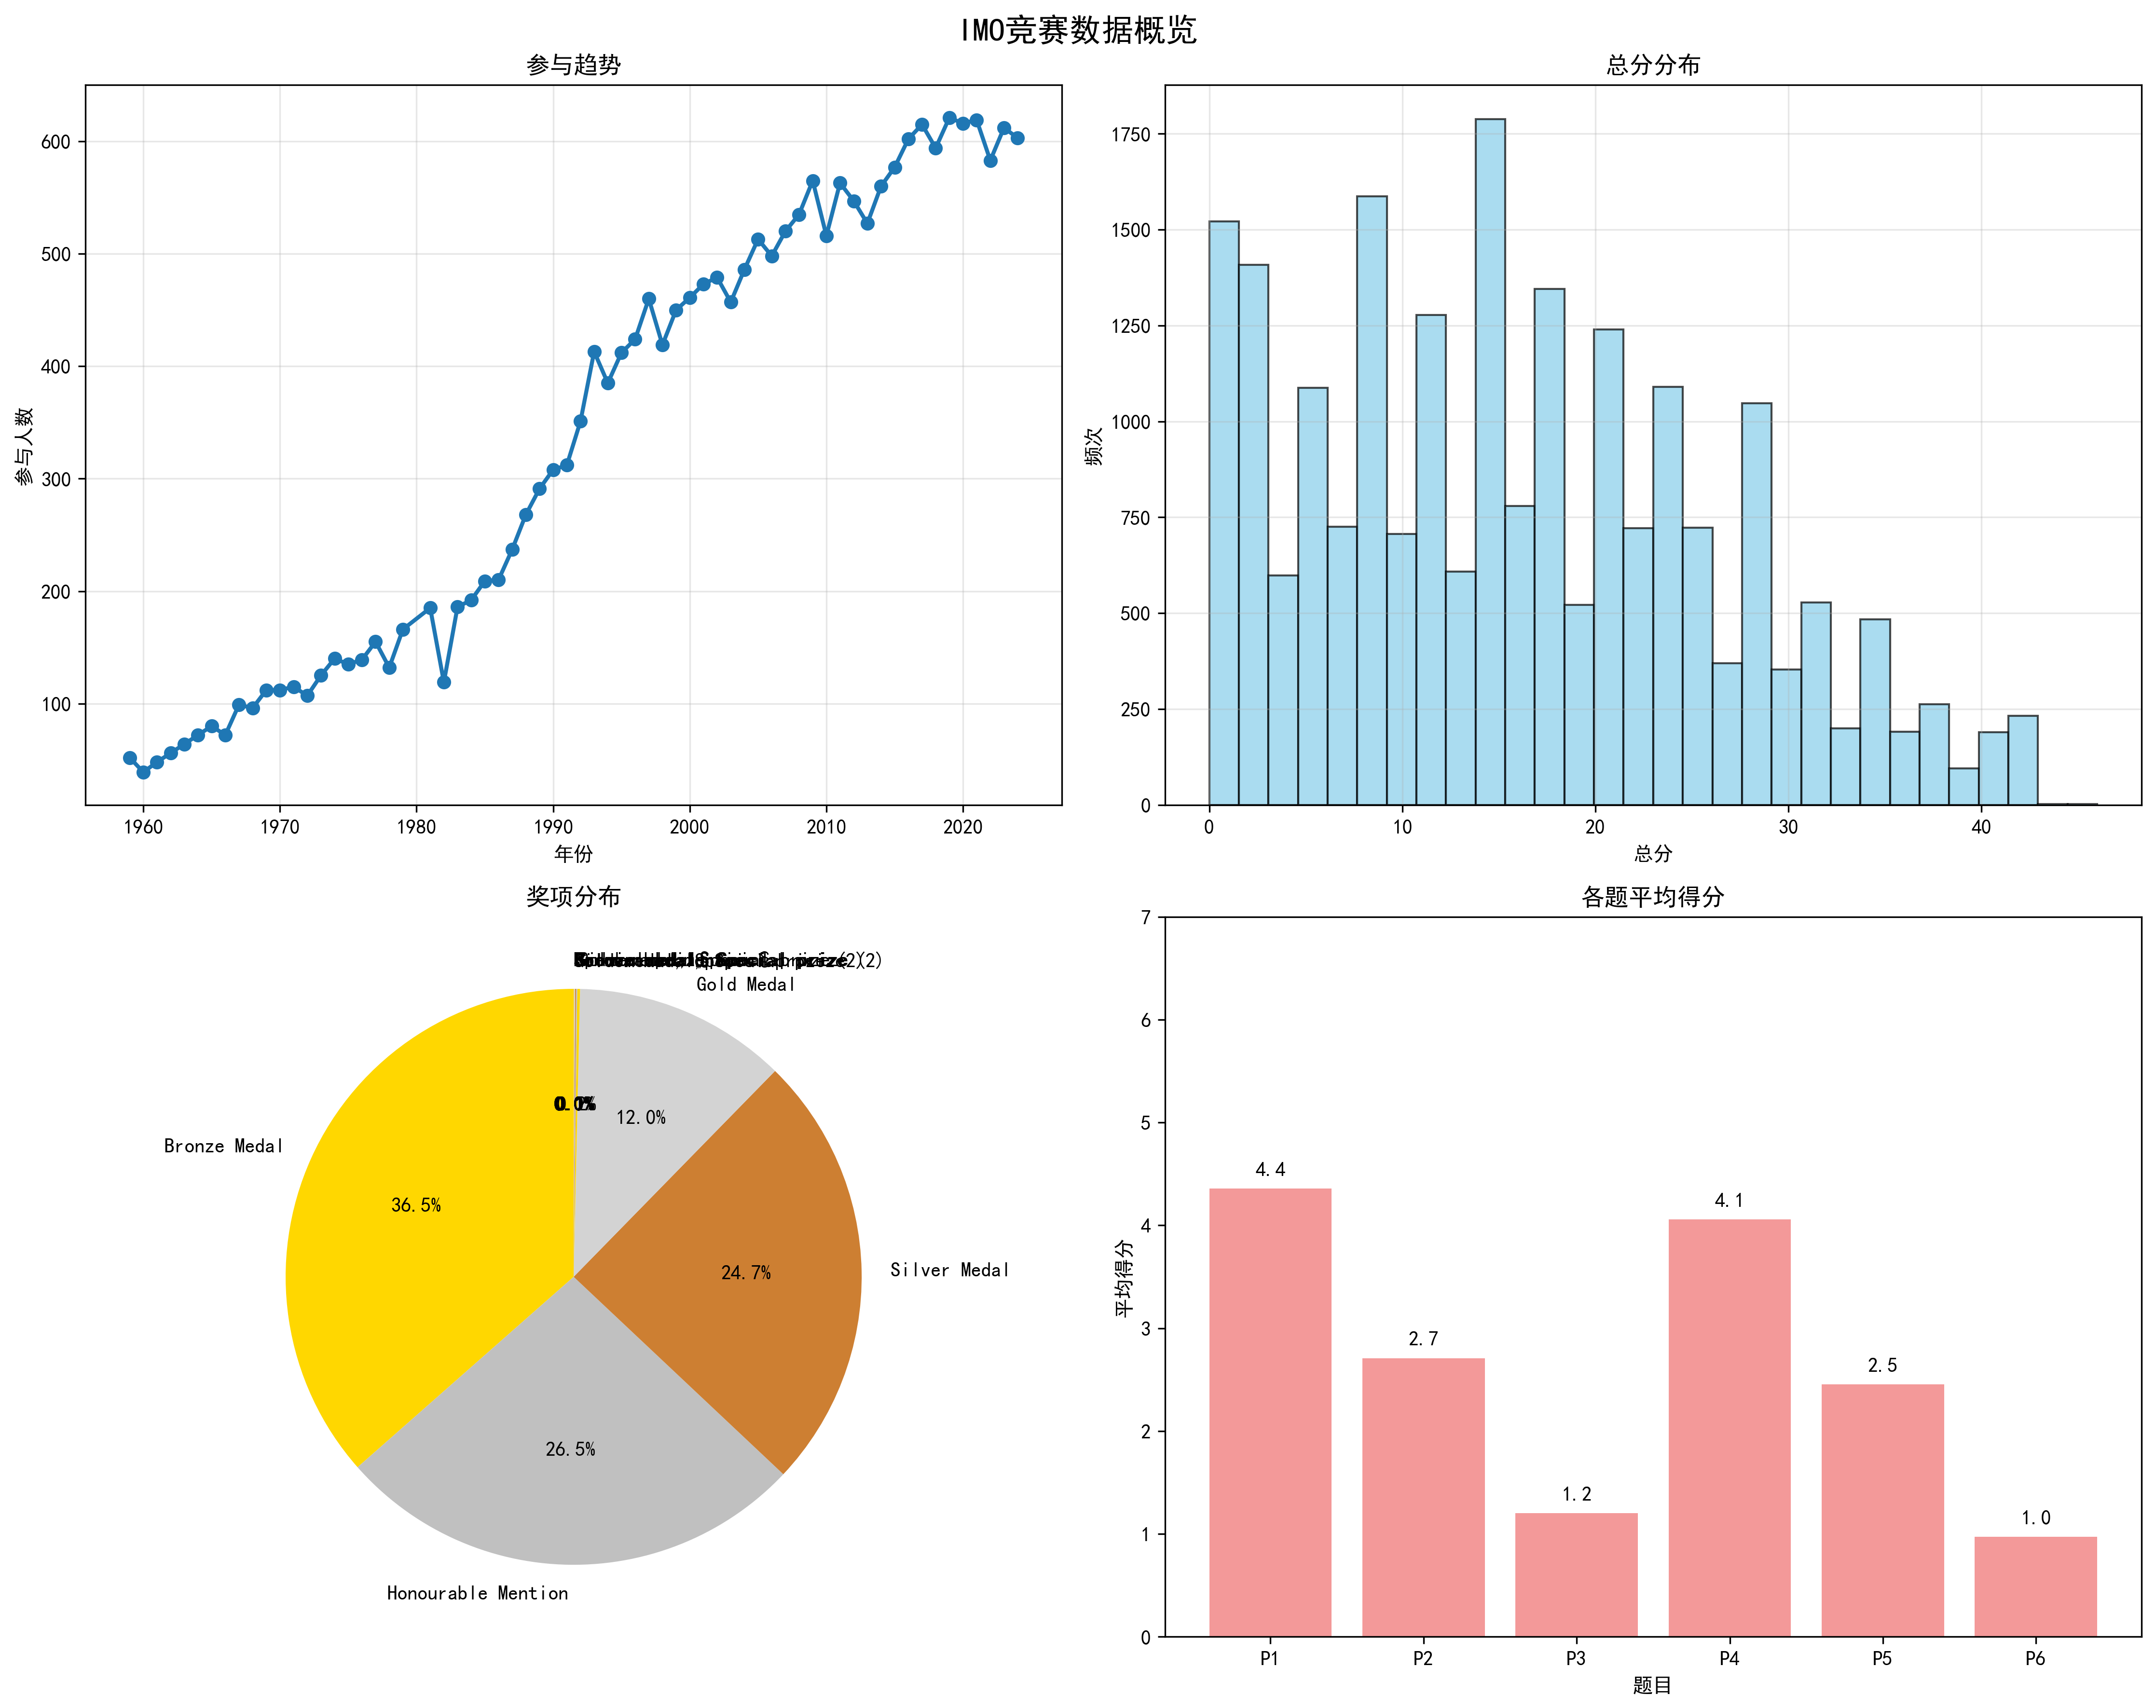
\includegraphics[width=\textwidth]{data_overview.png}
    \caption{IMO竞赛数据概览:(A)年度参赛人数趋势;(B)参赛者总分分布;(C)奖项分布比例;(D)各题平均得分。}
    \label{fig:data_overview}
\end{figure}

从图中可以获得以下初步洞察:
\begin{itemize}
    \item \textbf{参与趋势} (A): IMO的参与度经历了显著增长,尤其是在20世纪末期,近年来参赛人数稳定在较高水平,显示其全球影响力的成熟与稳固。
    \item \textbf{总分分布} (B): 参赛者总分呈明显的右偏分布,大量选手得分集中在中低分数段,而高分段人数较少,表明竞赛具有良好的区分度。
    \item \textbf{奖项分布} (C): 奖项构成呈现金字塔结构,金牌(8.1\%)最为稀少,其次是银牌(16.7\%)和铜牌(24.6\%),这一稳定的比例结构反映了IMO相对固定的评奖标准。
    \item \textbf{各题得分} (D): 题目难度存在显著差异。P1和P4的平均分远高于其他题目,而P3和P6的平均分最低,这揭示了IMO题目设计中可能存在的"位置效应"。
\end{itemize}

\section{多维度表现分析}
\subsection{国家竞争力分析}
国家是IMO竞赛的基本参与单位,对国家表现的分析是评估全球数学教育格局的核心。图\ref{fig:country_analysis}从多个角度比较了各国的竞争力。

\begin{figure}[H]
    \centering
    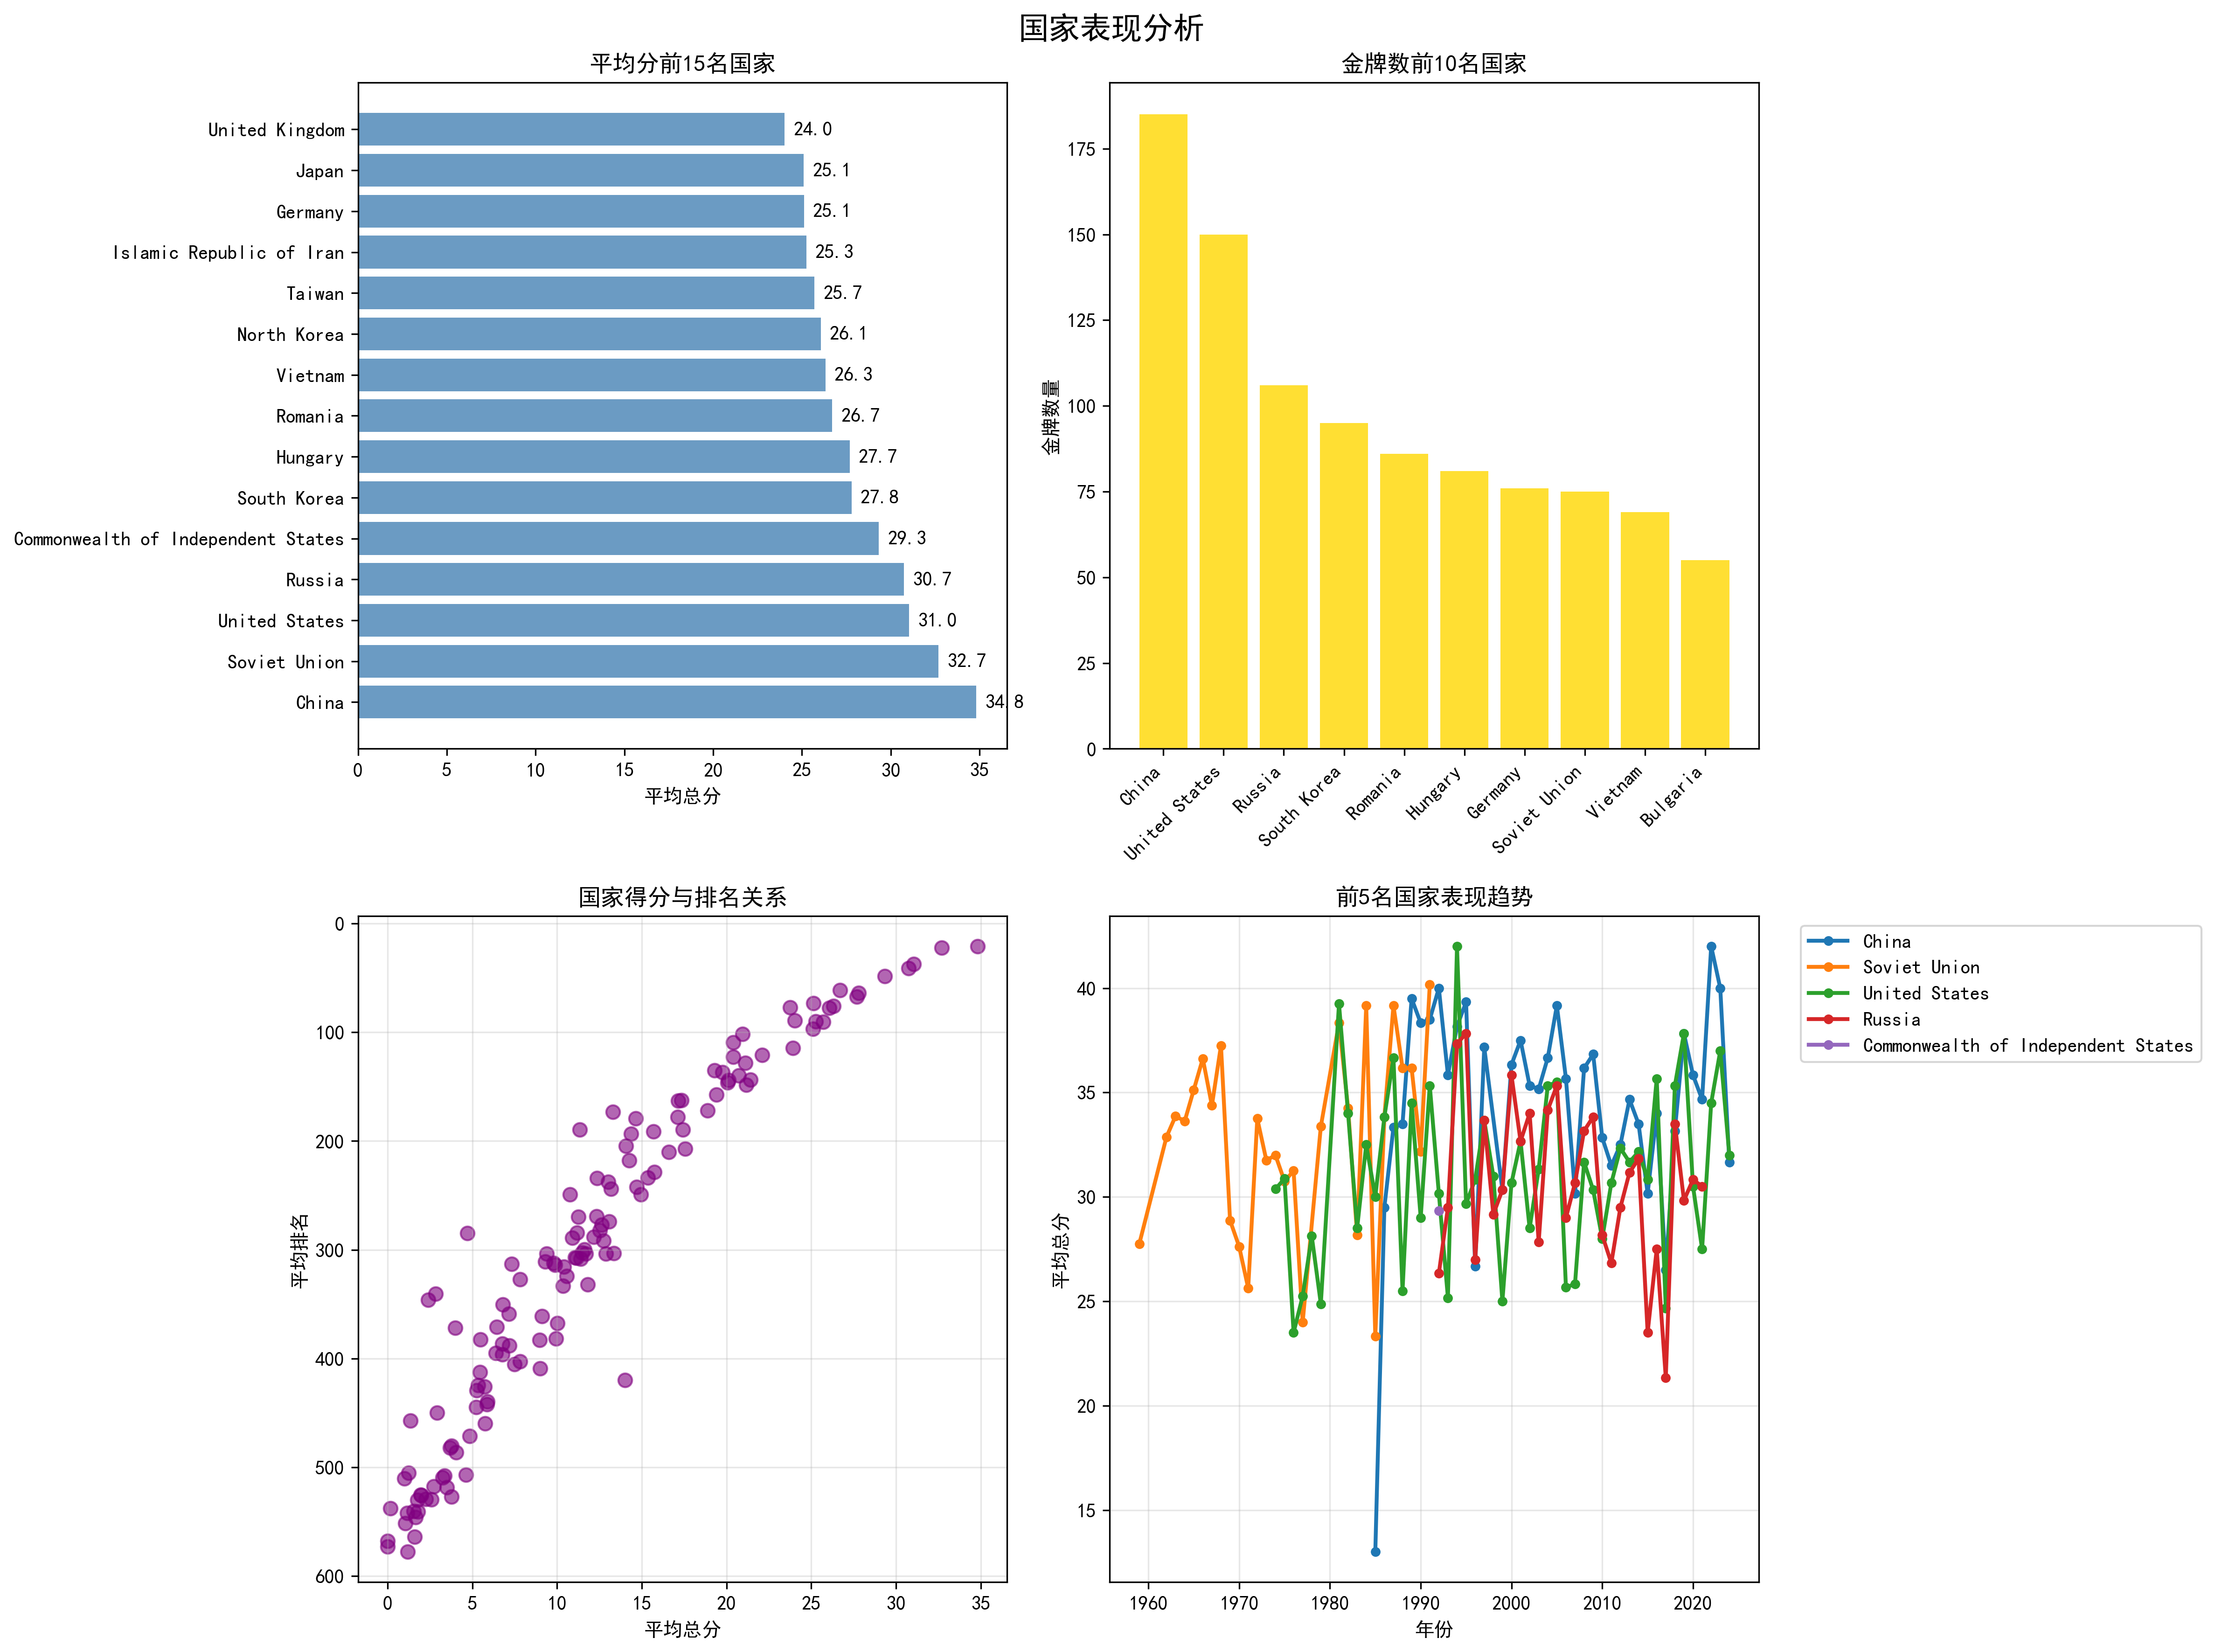
\includegraphics[width=\textwidth]{country_analysis.png}
    \caption{国家表现分析:(A)平均分排名前15国家;(B)金牌总数排名前15国家;(C)总分与排名的关系;(D)顶尖国家历年表现趋势。}
    \label{fig:country_analysis}
\end{figure}

分析图\ref{fig:country_analysis}可以得出以下结论:
\begin{itemize}
    \item \textbf{顶尖实力的集中性}:从平均分(A)和金牌总数(B)来看,少数国家构成了IMO的顶尖集团。特别是中国、美国、俄罗斯和韩国,在两项指标上均名列前茅,显示了其在数学精英教育方面的强大实力和深厚底蕴。
    \item \textbf{亚洲的崛起}:在平均分排名中,亚洲国家占据了多个席位,这与关于东亚数学教育优势的研究相符\cite{asian_mathematics_education,ma1999knowing}。这可能归因于文化传统、教育投入以及高效的选拔训练体系\cite{mathematical_olympiad_training}。
    \item \textbf{指标的一致性}:得分与排名的散点图(C)呈现出强烈的负相关,验证了竞赛评分系统的有效性。同时,(D)中顶尖国家表现的年度波动也表明,IMO的竞争是动态且激烈的。
\end{itemize}

\subsection{题目难度分析}
IMO竞赛的灵魂在于其精心设计的题目\cite{andreescu2006mathematical}。对题目难度的分析有助于理解竞赛的选拔机制。

\begin{figure}[H]
    \centering
    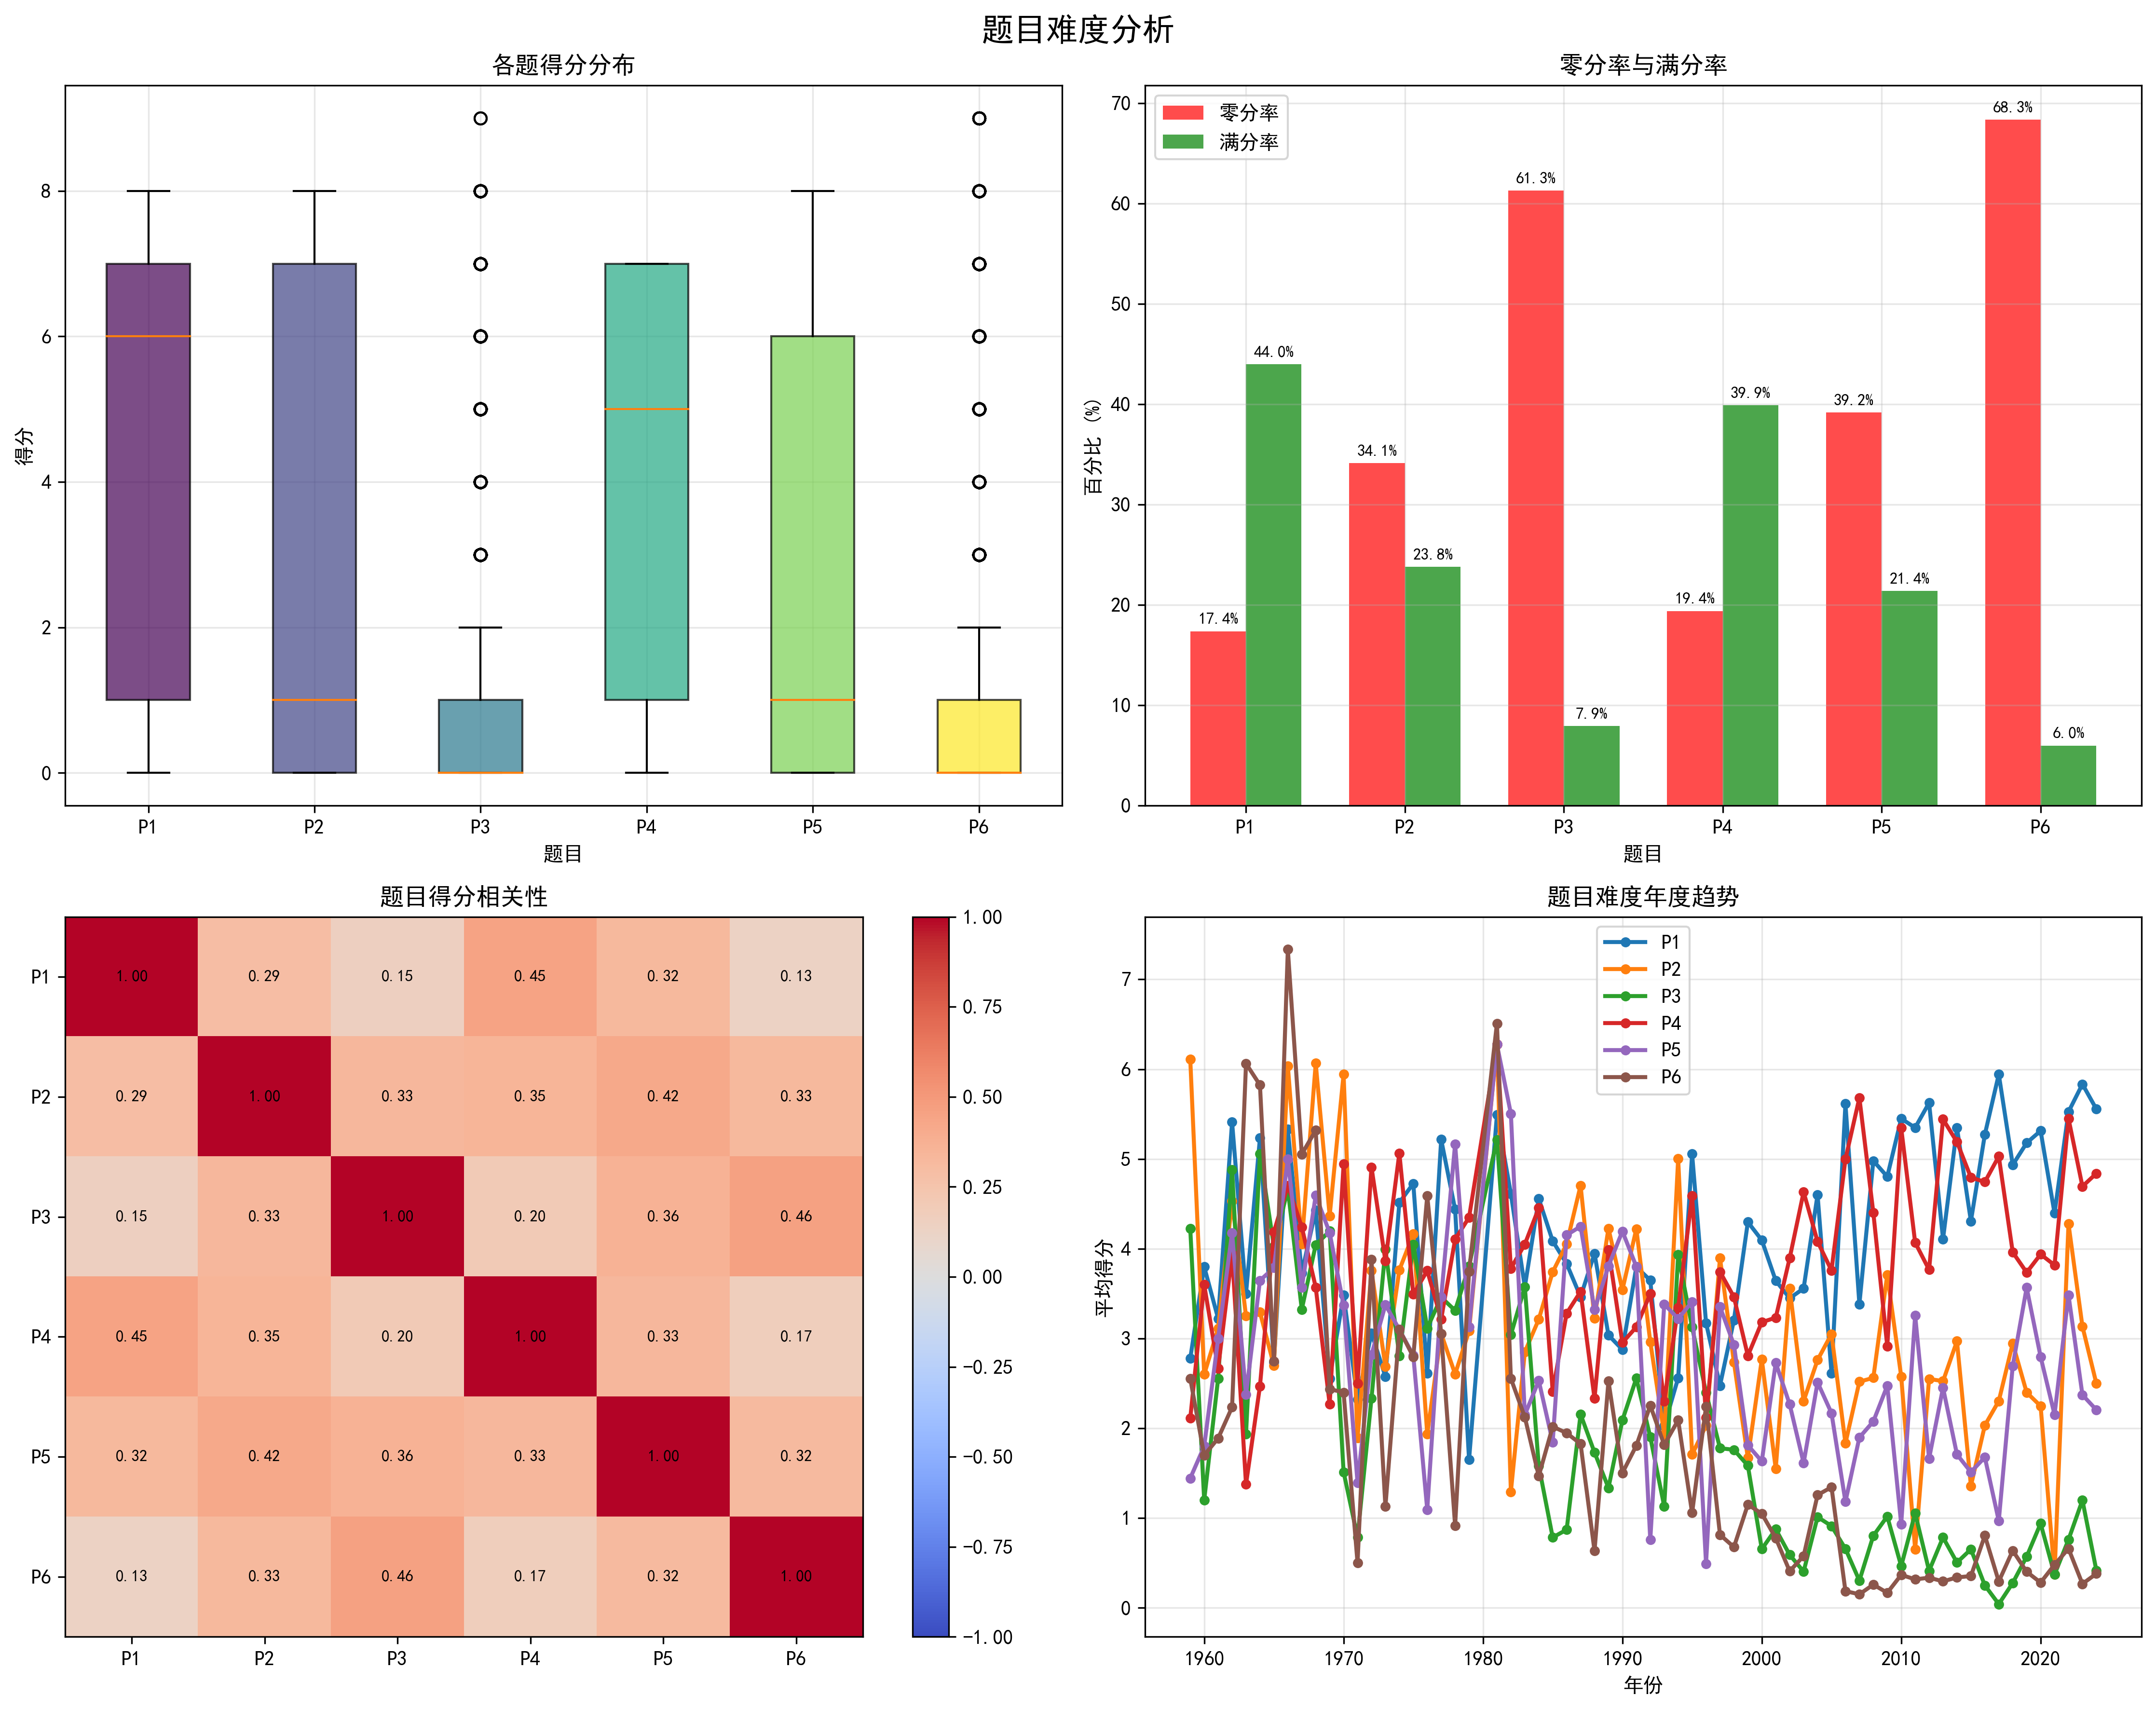
\includegraphics[width=\textwidth]{problem_difficulty.png}
    \caption{题目难度分析:(A)各题得分的小提琴图;(B)各题零分率与满分率;(C)题目得分相关性矩阵;(D)各题难度历年趋势。}
    \label{fig:problem_difficulty}
\end{figure}

图\ref{fig:problem_difficulty}揭示了IMO题目的设计哲学:
\begin{itemize}
    \item \textbf{显著的位置效应}:无论从得分分布(A)、零分/满分率(B)还是历史趋势(D)来看,P1和P4都显著比其他题目简单。它们作为每天的第一题,起到了让多数选手"热身"并建立信心的作用。
    \item \textbf{终极挑战}:P3和P6是竞赛中最难的题目,平均分最低,零分率最高。这些题目是区分顶尖高手、选拔具有非凡数学洞察力人才的关键,其内容常涉及数论、组合及高等几何等艰深领域\cite{rosen2019handbook,coxeter1961introduction}。
    \item \textbf{能力的一致性}:相关性矩阵(C)显示,所有题目得分之间均存在正相关,这表明参赛者在不同数学领域的表现具有一定的一致性,反映了其综合数学素养。
\end{itemize}

\subsection{奖项与评奖机制分析}
奖项是衡量参赛者成就的直接标志。对奖项的分析可以反映竞赛的评价标准。

\begin{figure}[H]
    \centering
    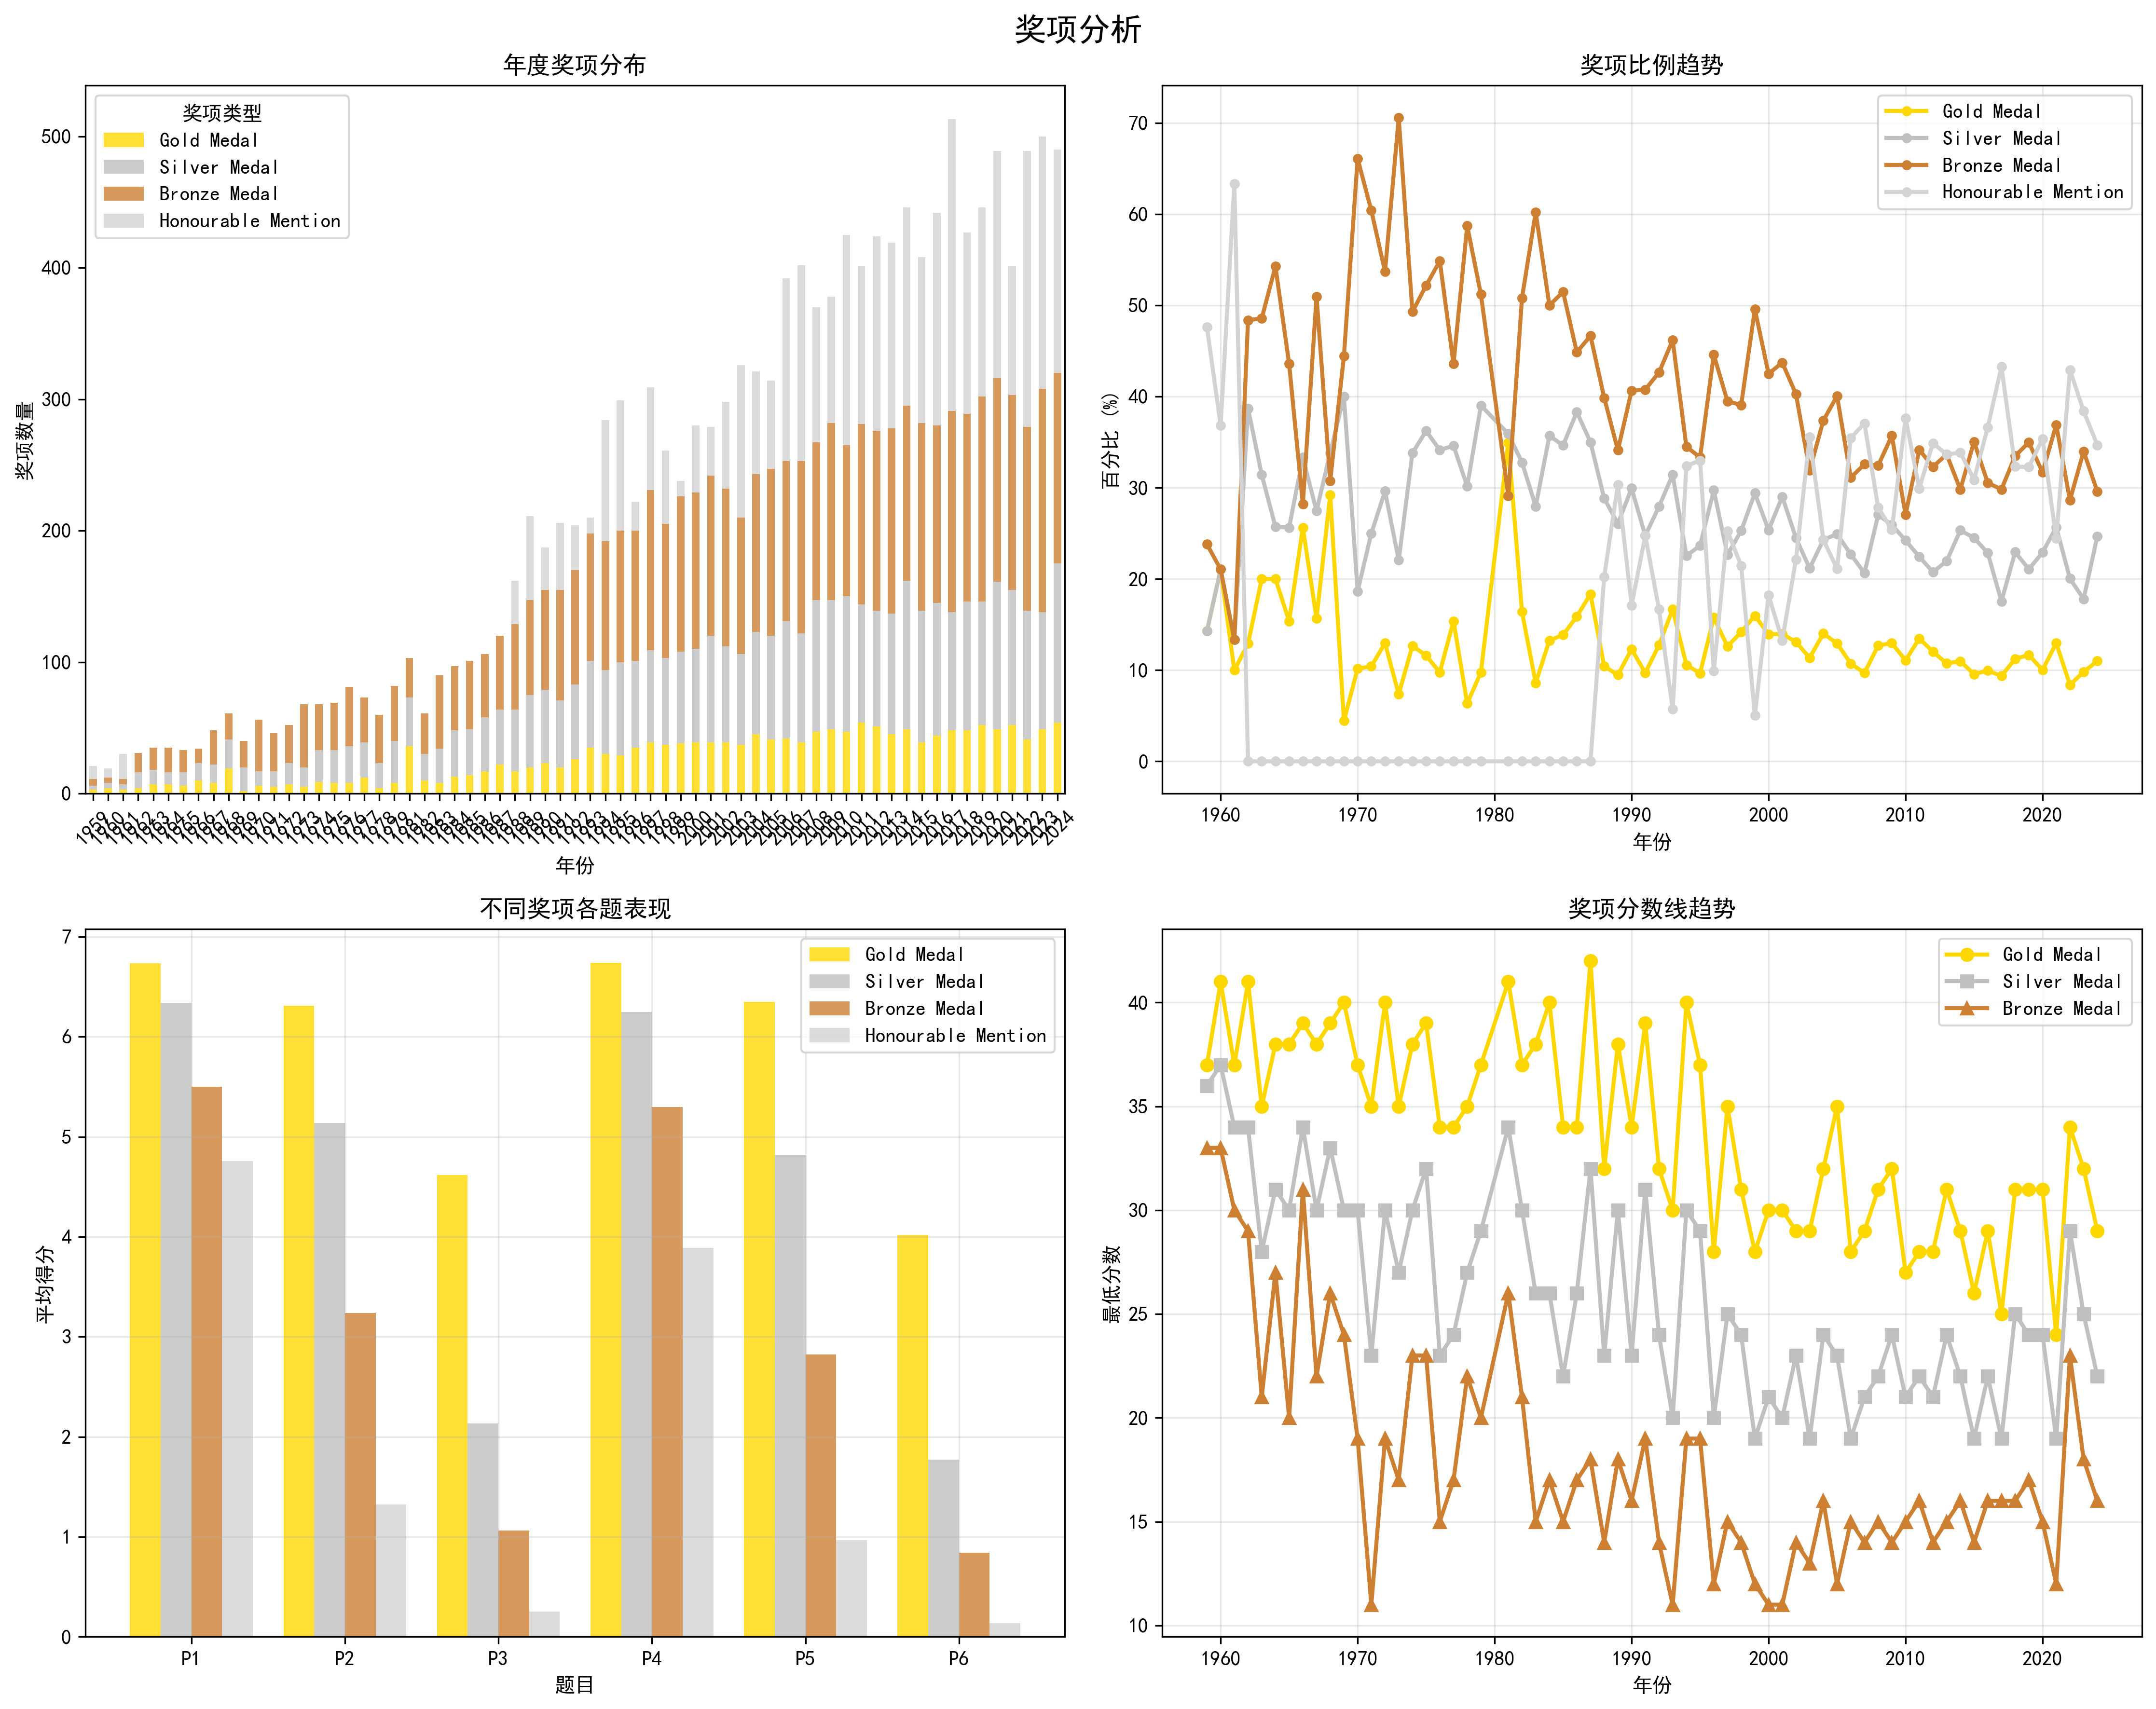
\includegraphics[width=\textwidth]{award_analysis.png}
    \caption{奖项分析:(A)各奖项人数占比;(B)各奖项人数历年变化;(C)各奖项获得者在各题上的平均表现;(D)各奖项分数线历年趋势。}
    \label{fig:award_analysis}
\end{figure}

从图\ref{fig:award_analysis}中我们观察到:
\begin{itemize}
    \item \textbf{稳定的评奖比例}:尽管每年的题目难度和参赛者水平有波动,但金、银、铜牌的获奖比例基本遵循1:2:3的原则,总获奖人数约占总参赛人数的一半。这种相对稳定的比例说明IMO采用的是一种相对评价而非绝对分数线的评奖体系。
    \item \textbf{奖项的区分度}:不同等级奖项获得者在所有6道题目上的表现(C)呈现出清晰的梯度,这再次证明了竞赛题目设计的有效性。值得注意的是,即使是金牌得主,在P6上的平均分也远低于满分,凸显了该题目的极高挑战性。
\end{itemize}

\subsection{地区差异分析}
将国家按地理位置划分为地区,可以帮助我们从更宏观的视角审视全球数学教育的不均衡发展。

\begin{figure}[H]
    \centering
    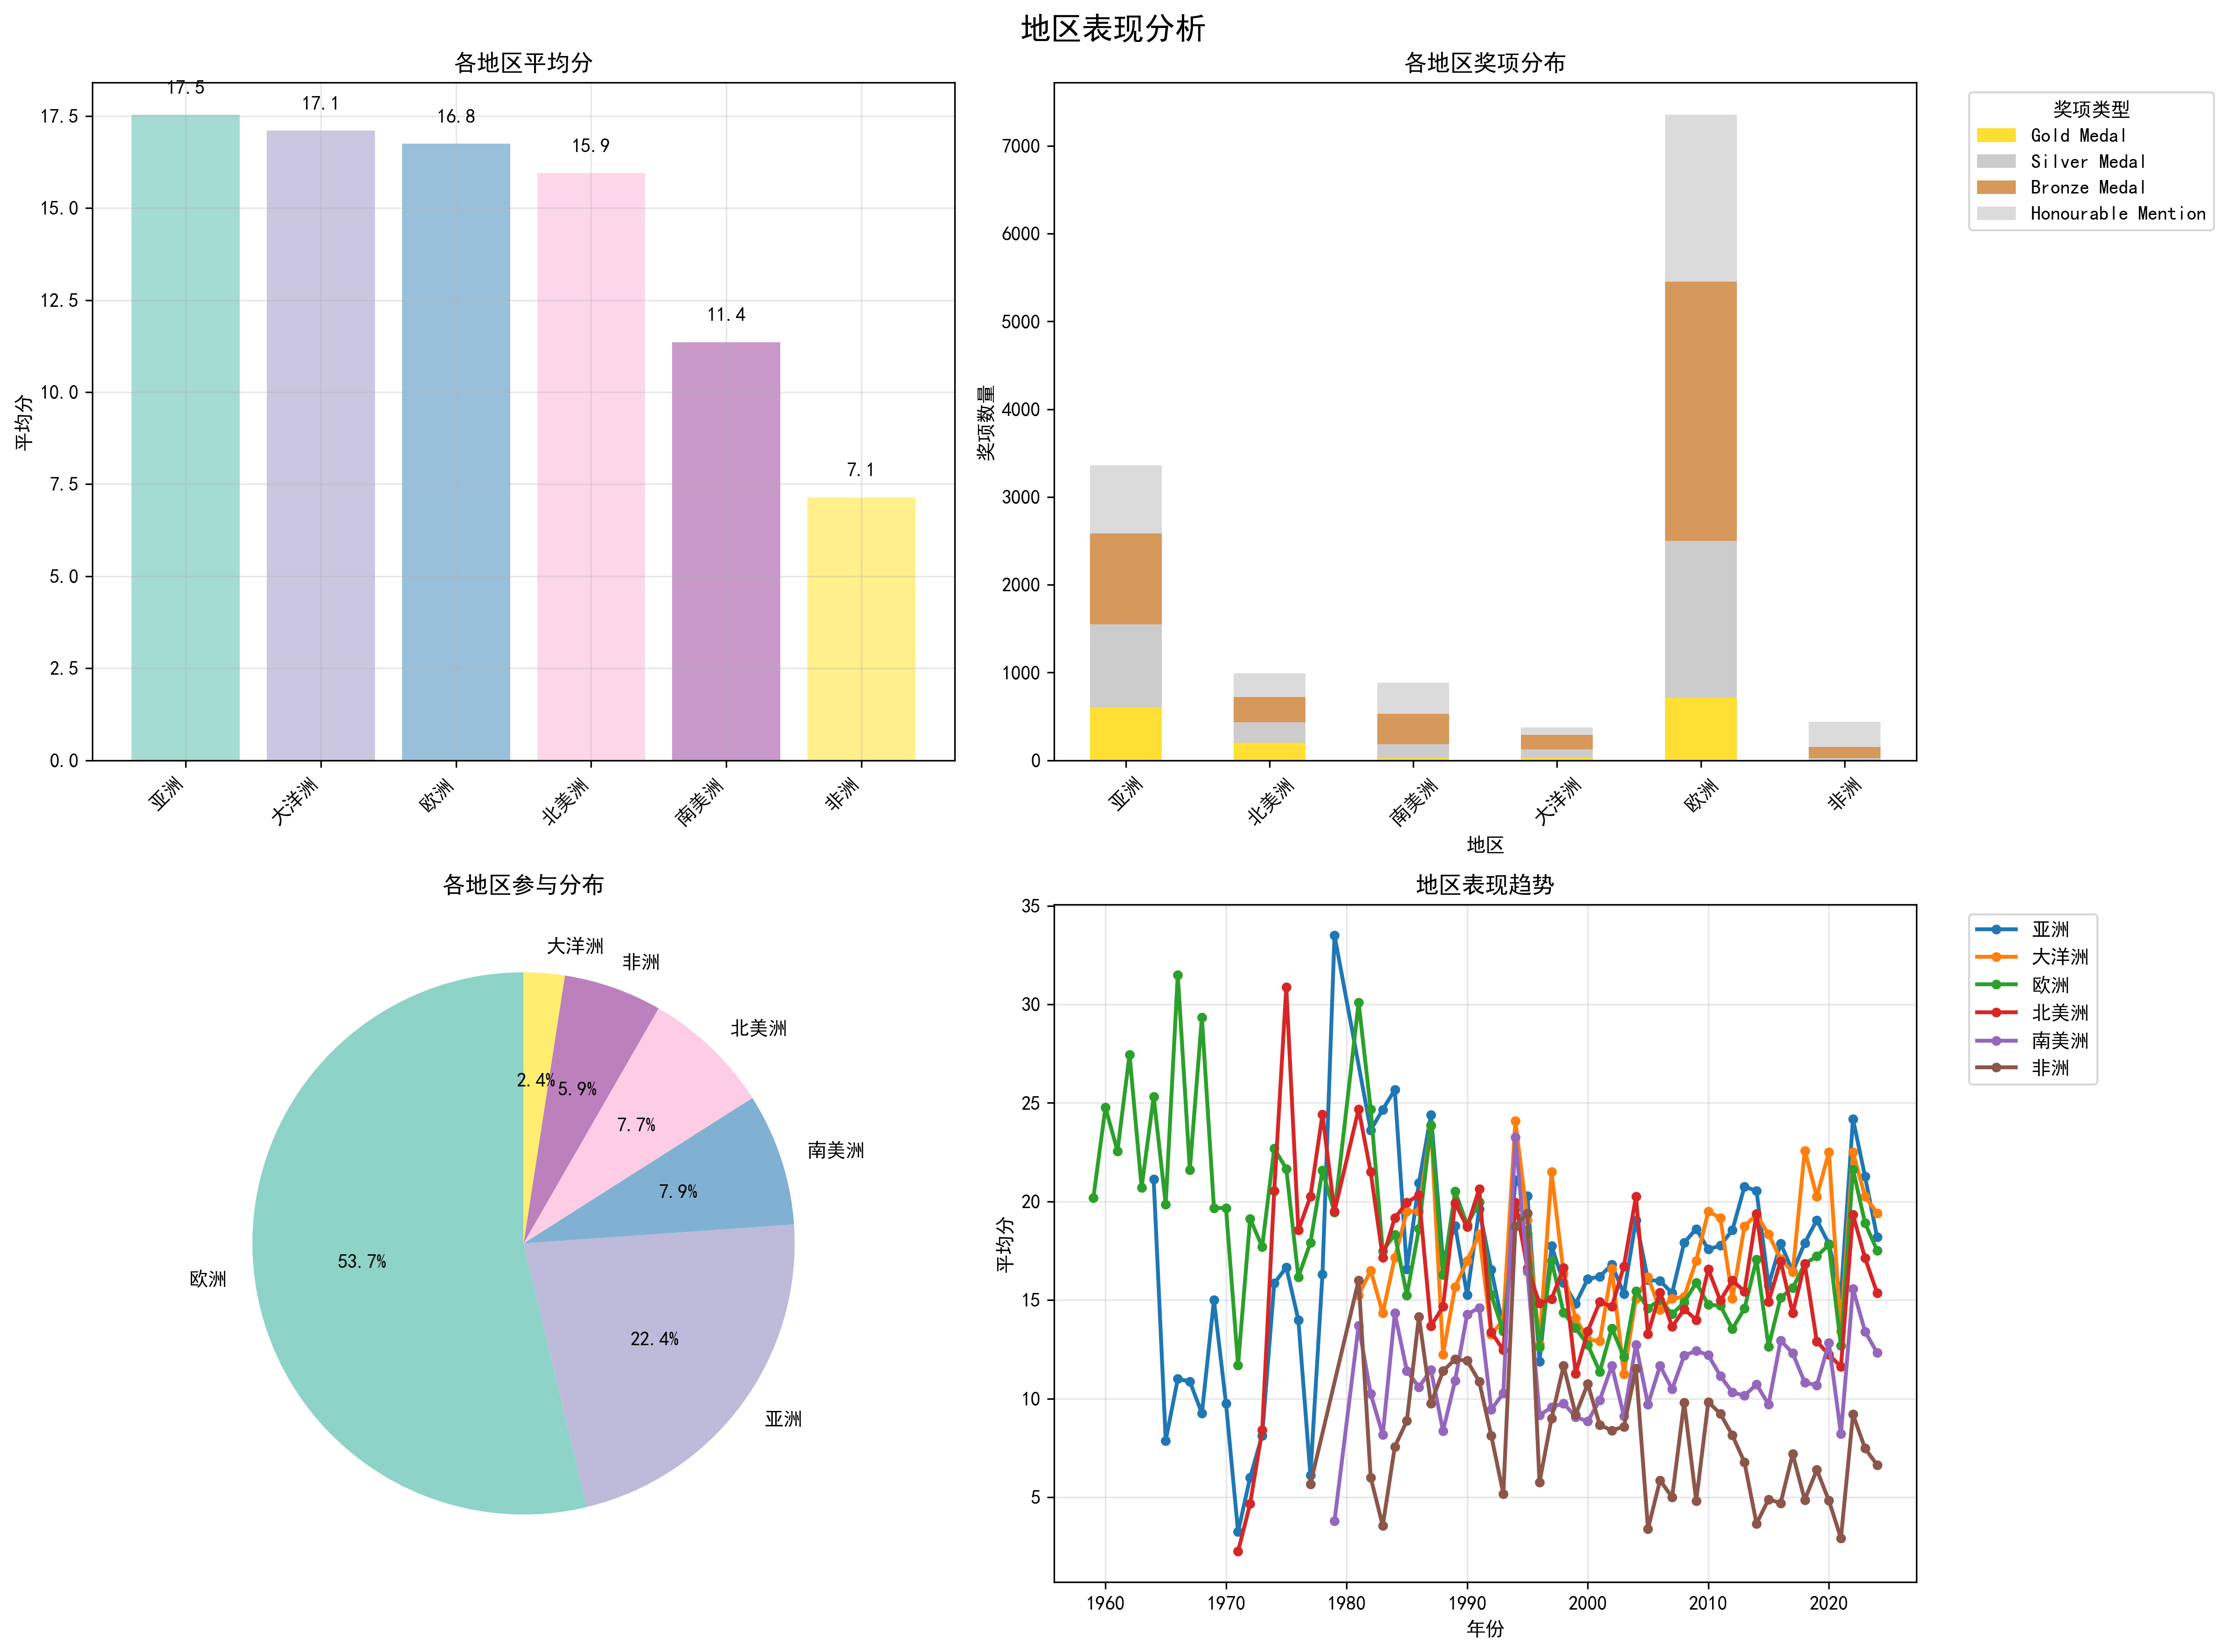
\includegraphics[width=\textwidth]{regional_analysis.png}
    \caption{地区表现分析:(A)各地区总参与人数;(B)各地区平均分;(C)各地区奖牌分布;(D)各地区平均分历年趋势。}
    \label{fig:regional_analysis}
\end{figure}

地区层面的分析(图\ref{fig:regional_analysis})揭示了显著的差异:
\begin{itemize}
    \item \textbf{欧洲的广泛参与}:欧洲是IMO参与度最高的地区,这得益于其悠久的数学传统和早期参与。
    \item \textbf{大洋洲与亚洲的优异表现}:尽管参与人数不多,大洋洲的平均分却最高。而亚洲则在维持较高参与度的同时,取得了优异的平均表现,其近年来的上升趋势(D)尤为明显。
    \item \textbf{发展的挑战}:非洲和南美洲的参与度和平均表现均相对较低,这可能反映了这些地区在基础教育资源、师资力量和拔尖人才培养体系方面面临的挑战。这一发现与TIMSS等其他国际教育评估的结果具有一致性\cite{timss_trends}。
\end{itemize}


\section{深入讨论}

\subsection{全球竞争格局的动态演化}

本研究的数据揭示了一幅动态的全球数学精英教育竞争图景。如果说20世纪的IMO见证了苏联和东欧集团的强大实力,那么进入21世纪,竞争格局则呈现出显著的"东移"趋势。以中国为代表的东亚国家,自上世纪八九十年代参赛以来,迅速崛起为一股不可忽视的力量。如图\ref{fig:country_analysis}D所示,中国队成绩的稳定性和高水平,以及韩国队的紧随其后,共同塑造了当前的竞争格局。这一现象并非偶然,它与东亚社会普遍重视教育、强调勤奋的文化传统,以及国家层面系统性的奥赛选拔与培训体系密切相关\cite{asian_mathematics_education,mathematical_olympiad_training}。

与此同时,以美国为代表的传统强国依然保持着强大的竞争力。与东亚模式不同,美国的优势可能更多源于其高质量、多样化的高等教育资源,以及鼓励创新和探索的学术氛围,能够吸引和培养顶尖的数学人才。因此,IMO的顶尖竞争,实际上是不同教育哲学和培养模式之间的一场"对话"。

\subsection{IMO题目设计的教育学蕴涵}

本研究对题目难度的分析,证实了IMO并非一个单纯的数学知识测验,而是一个精心设计的认知评估工具。其"入口(P1/P4)- 区分(P2/P5)- 挑战(P3/P6)"的难度梯度设计,蕴含着深刻的教育学考量。

"入门题"的存在,保证了绝大多数有才华的参赛者都能获得一部分分数,避免了"零分"打击可能带来的挫败感,保护了参赛者的竞赛热情。而"挑战题"则精准地服务于IMO的核心目标——"识别最高水平的数学天才"\cite{gifted_mathematics_education}。这些题目往往无法通过常规的解题套路解决,需要参赛者展现出非凡的直觉、深刻的洞察力和原创性的构造能力,这正是杰出数学家所必备的关键特质\cite{problem_solving_strategies}。

因此,IMO的题目设计本身就是一套宝贵的教育资源。中学数学教师可以借鉴其设计思想,在日常教学中引入不同层次的开放性问题,从而更好地激发学生的思维潜力,实现从"解题"到"创造"的跨越。

\subsection{作为教育公平透镜的IMO}

尽管IMO聚焦于精英选拔,但其数据同样能够折射出全球教育公平的现状。图\ref{fig:regional_analysis}所揭示的地区间巨大差异,是全球"教育鸿沟"的一个缩影。非洲和南美洲等地区在参与度和表现上的双重落后,凸显了经济发展水平、教育资源投入对一个国家拔尖创新人才培养能力的深刻影响。

然而,数据也带来希望。越南、伊朗等发展中国家在IMO赛场上的不俗表现说明,通过国家层面的战略重视和持续投入,后发国家完全有可能在国际智力竞争中实现突破。这为其他发展中国家提供了宝贵的经验:精英教育的发展并非遥不可及,关键在于制定符合国情的、长期的发展战略。

\section{结论}

\subsection{主要研究结论}
本研究通过对IMO逾60年的历史数据进行量化分析,系统地揭示了其在全球数学教育领域的多重映像。主要结论可归纳为:
\begin{enumerate}
    \item \textbf{全球格局:从欧洲中心到多极竞争。} IMO早期由东欧国家主导,但随着全球参与度的扩大,逐渐形成了以美国、中国、俄罗斯、韩国等国为代表的多极竞争格局,特别是亚洲国家的群体性崛起是近三十年最显著的特征。
    \item \textbf{题目设计:科学分层的选拔工具。} IMO的题目设计并非难度均匀分布,而是遵循了"入口-区分-挑战"的科学分层模式。P1/P4保证了参与度,而P3/P6则成为选拔顶尖天才的终极试金石,有效服务于其核心选拔目标。
    \item \textbf{评价体系:相对稳定的精英标尺。} IMO的评奖机制通过相对比例而非绝对分数来授予奖项,使其能够在不同年份、不同难度试卷下,保持评价标准的一致性,稳定地识别出全球最顶尖的约8\%的数学苗子。
    \item \textbf{地区差异:教育不平等的缩影。} 全球五大洲在IMO的参与度和表现上存在显著差异,这不仅反映了各国数学教育水平,也在一定程度上折射出更深层次的经济发展、教育投入和文化传统差异。
\end{enumerate}

\subsection{研究的意义与启示}
本研究的发现对数学教育政策制定者、研究者和实践者具有多重启示:
\begin{itemize}
    \item \textbf{对教育政策:} 各国在IMO上的表现可作为其基础数学教育,特别是英才教育成效的一个参考指标。亚洲国家的成功经验,如对基础知识的重视、系统性的选拔与训练,值得其他国家借鉴\cite{asian_mathematics_education}。同时,地区间的巨大差距也提醒国际社会需关注并支持发展中地区的数学教育。
    \item \textbf{对数学教育研究:} IMO数据为数学问题解决\cite{schoenfeld1985mathematical}、天才发展\cite{gifted_mathematics_education}、性别差异\cite{gender_mathematics_performance}等经典研究课题提供了宝贵的真实世界数据。未来的研究可在此数据集上进行更复杂的因果推断或预测建模。
    \item \textbf{对竞赛实践:} 本研究验证了IMO现有题目设计和评奖机制的科学性。组织者可继续优化题目设计,以适应不断变化的教育环境,并探索如何利用竞赛进一步促进全球数学教育的公平与发展。
\end{itemize}

\subsection{局限性与未来展望}
本研究作为一项探索性分析,也存在一些局限性。首先,数据集中缺少参赛者的个人背景信息(如性别、学习背景),限制了更细粒度的分析,例如无法直接探讨性别在顶尖数学表现中的差异问题\cite{gender_mathematics_performance}。其次,本研究主要采用描述性统计和可视化,未来的工作可以引入更高级的统计模型(如时间序列模型来预测国家表现的演化,或多层线性模型来分离国家和个人层面的影响因素)。最后,将IMO数据与其他国际评估(如PISA, TIMSS)数据进行个体或国家层面的融合分析,可能会产生更有价值的洞见,更全面地评估普及教育与精英教育的关系。

未来,我们期望构建一个交互式的数据探索平台,让全球的教育研究者和爱好者都能方便地探索IMO数据,共同挖掘其更深层次的价值。

\section{致谢}
本研究的顺利完成得益于TidyTuesday社区和IMO官方组织提供的高质量公开数据。同时,感谢南开大学提供的学术资源和研究环境。最后,感谢所有为国际数学教育事业做出贡献的前辈和同仁。

\clearpage
\phantomsection
\addcontentsline{toc}{section}{参考文献}
\renewcommand{\bibname}{参考文献}
\bibliography{reference}

\end{document} 